\chapter{การวิเคราะห์และออกแบบระบบ}

การวิเคราะห์และออกแบบระบบก่อนดำเนินการจริงเป็นอีกหนึ่งขั้นตอนที่มีความสำคัญมาก เพราะการวิเคราะห์และออกแบบระบบนั้นเป็นการกระทำที่ทำให้ผู้พัฒนาเห็นรายละเอียดส่วนย่อยของงานทั้งหมด เพิ่มประสิทธิภาพในการวางแผน การทำงาน และยังช่วยลดปัญหาที่อาจจะเกิดขึ้นในระหว่างพัฒนา เพื่อให้ระบบมีความสมบูรณ์มากยิ่งขึ้น เนื่องจากการวิเคราะห์และออกแบบระบบนั้นจะช่วยให้ให้บริการ จัดการทรัพยากรได้อย่างคุ้มค่าและตรงตามความต้องการของระบบ

การวิเคราะห์และออกแบบแอปพลิเคชันสแกนอาหาร ในบทนี้จะแบ่งออกเป็น 6 ข้นตอนเพื่อให้เห็นการดำเนินงานอย่างมีระบบ ในหัวข้อแรกจะนำเสนอภาพรวมของระบบ ก่อนจะนำเสนอเอกสารแสดงความต้องการของระบบซึ่งจะทำให้เห็นที่มาของเพจต่าง ๆ ในขั้นตอนของการออกแบบในหัวข้อที่สาม ส่วนหัวข้อที่เหลือจะแสดงแผนภาพการการทำงานของระบบโดยใช้ UML diagram ซึ่งประกอบไปด้วย Use Case, Class และ Sequence Diagram เพื่อแสดงรายละเอียดของระบบก่อนนำไปเขียนคำสั่งด้วยภาษาโปรแกรมในบทต่อไป

\begin{enumerate}[label=3.\arabic*]
	\item โครงสร้างภาพรวมของระบบ (System Architecture) เป็นการออกแบบภาพรวมและเทคโนโลยีของระบบ
	\item System Requirements คือ ความต้องการหรือสิ่งที่ระบบควรจะทำ หรือหน้าที่หลักของ
	ระบบที่จะต้องทำ
	\item User Interface Design เป็นการออกแบบส่วนต่อประสานกับผู้ใช้
	\item Use Case Diagram เป็นแผนภาพที่ใช้แสดงให้ทราบว่าระบบทำงานหรือมีหน้าที่ใดบ้าง
	\item Class Diagram เป็นแผนภาพที่ใช้แสดง Class และความสัมพันธ์ระหว่าง Class
	\item Sequence Diagram เป็นแผนภาพที่ใช้แสดงให้เห็นถึงการตอบโต้ข้อมูลระหว่างคลาส เรียงตามลำดับของเวลาที่เกิดเหตุการณ์จากน้อยไปมาก
\end{enumerate}	

\section{โครงสร้างการทำงานข้อระบบ}
 ระบบแอปพลิเคชัน What is that มีโครงสร้างการทำงานดังรูปที่ 3.1
   	\begin{figure}[H]
   		\centering
   		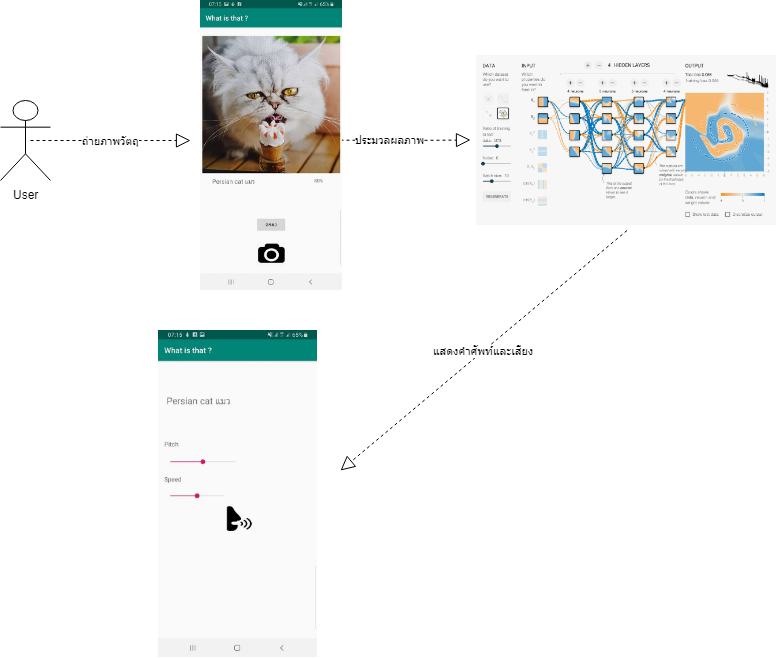
\includegraphics[width=\textwidth]{Figures/3/architecture/31.png}
   		\caption{โครงสร้างการทำงานข้อระบบ}
   		\label{Fig:architecture}
   	\end{figure}
   
	 		จากรูปที่ \ref{Fig:architecture} สามารถอธิบายโครงสร้างการทำงานของระบบได้ดังนี้ ผู้ใช้งานต้องทำการถ่ายต้องการ ระบบจะนำภาพไปเปรียบเทียบกับข้อมูลที่ผ่านกระบวนการประมวลผลภาพ
 จากนั้นระบบจะแสดงคำศัพท์ภาษาอังกฤษของภาพนั้นๆแล้วแปลงข้อความที่ได้เป็นเสียงพูด 
   

\section{System Requirements}
		\subsection{Functional Requirements} 
แอปพลิเคชัน What is that แบ่งตามประเภทผู้ใช้งานดังนี้ 
\begin{enumerate}
		\item ผู้ใช้งาน
			\begin{itemize}[label={--}]
				\item สามารถระบุภาพภ่ายได้
				\item สามารถดูคำศัพท์และคำแปลได้
				\item สามารถฟังเสียงของคำศัพท์นั้นได้่
				\item สามารถเลือกระดับความเร็วในการออกเสียงได้ 
				\item สามารถลือกโทนเสียงได้
			\end{itemize}
			\end{enumerate}

		\subsection{Non-functional Requirements}
		\begin{enumerate}
		\item แอนดรอยด์แอปพลิเคชัน
		\begin{itemize}[label={--}]
			\item  แอปพลิเคชันสามารถวิเคราะห์ภาพได้ภายในระยะเวลา 1 วินาที 
			\item  แอปพลิเคชันมีเสียงรองมากกว่า 1 ภาษา
		
		\end{itemize}
	\end{enumerate}
	
\section{User Interface Design}
ในการออกแบบ User Interface Design ของแอปพลิเคชันสแกนอาหาร ออกแบบมาให้มีลักษณะที่ใช้งานง่ายเพียงแค่ไม่กี่ขั้นตอน โดยสามารถโต้ตอบกับผู้ใช้ได้ 
\begin{itemize}[label={--}]

\item การออกแรกของแอพพลิเคชัน

				\begin{figure}[H]
					\centering
					
\includegraphics[width=0.2\textwidth]{Figures/3/UIDESIGN/main.png}
					\caption{หน้าแรก}
					\label{Fig:1}
				\end{figure}
				จากภาพที่ \ref{Fig:1}แสดงหน้าหลักและอธิบายรายละเอียดของตัวแอพพลิเคชั่น
			\end{enumerate}
		\end{itemize}

				\newpage

				\begin{itemize}[label={--}]

\item การออกแบบหน้าจอวิเคราะห์ภาพ 
	\begin{figure}[H]
					\centering
					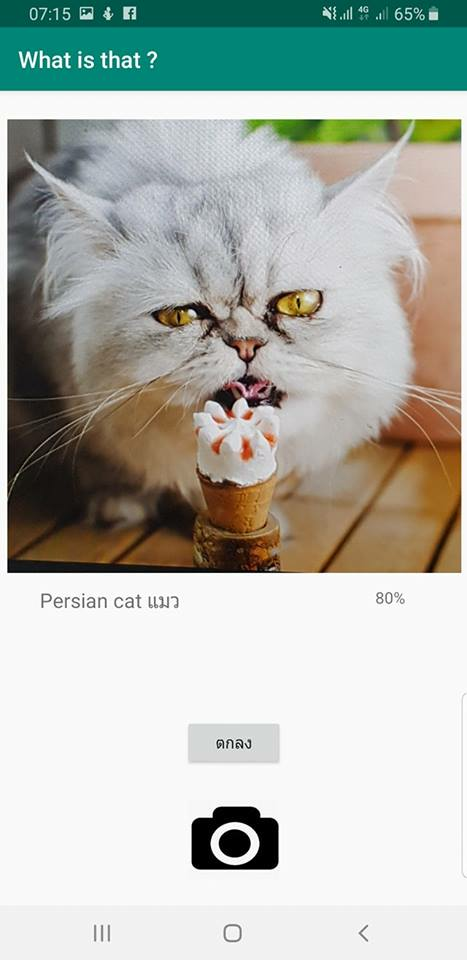
\includegraphics[width=0.2\textwidth]{Figures/3/UIDESIGN/pic.png}
					\caption{หน้าระบุถาพถ่ายที่เลือก}
					\label{Fig:2}
				\end{figure}
				จากภาพที่ \ref{Fig:2} เมื่อผู้ใช้ทำการกดที่ปุ่ม ตกลง ระบบจะทำการวิเคราห์ภาพแล้วแสดงคำศัพท์ภาษาอังกฤษของภาพนั้นๆ หรือกดที่รูปกล้องเพื่อกลับไปถ่ายภาพวัตถุใหม่อีกครั้ง
			\end{itemize}
	\begin{itemize}[label={--}]
\item การออกแบบหน้าจอเสียงพูด 
				\begin{figure}[H]
								\centering
								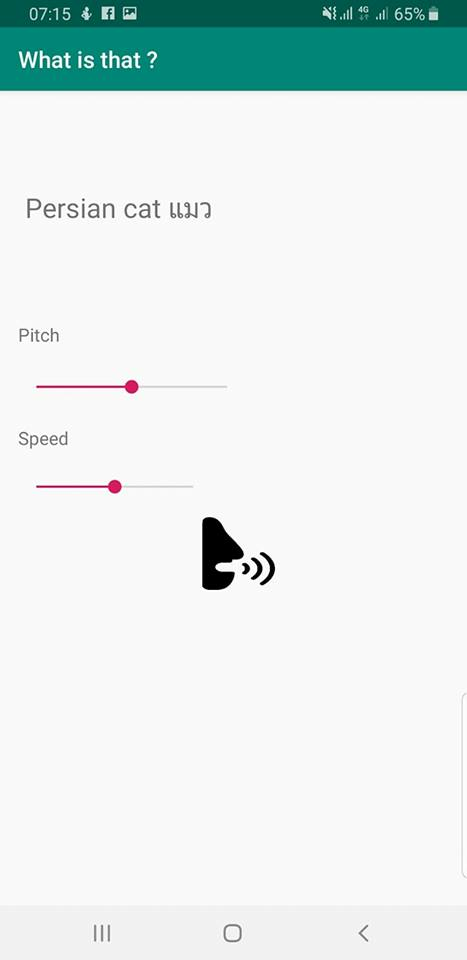
\includegraphics[width=0.2\textwidth]{Figures/3/UIDESIGN/speak.png}
								\caption{หน้าจอ แดชบอร์ด}
								\label{Fig:5}
							\end{figure}
							จากภาพที่ \ref{Fig:5} ในหน้านี้จะนำคำศัพท์ที่ได้มาประมวลผล และสามาถกดเพื่ออ่านออกเสียงคำศัพท์นั้นเป็นภาษาอังกษได้ อีกทั้งยังสมารถเลือกความเร็วในการอ่านออกเสียงได้เพื่อให้ผู้ใช้สามารถฟังได้ง่ายขึ้น
						\end{itemize}
							\newpage

\begin{itemize}[label={--}]

								
									\end{itemize}


										\newpage

\section{Use Case Diagram}
	Use Case Diagram เป็นแผนผังเพื่อแสดงฟังก์ชันแสดงการทำงานของระบบโดยรวม แสดงส่วนประกอบในระบบและกิจกรรมที่เกิดขึ้นในระบบซึ่งในระบบระบบกองทุนเงินให้กู้ยืมเพื่อการศึกษา คณะวิทยาศาสตร์ มหาวิทยาลัยอุบลราชธานี ผู้ใช้จำเป็นต้องเข้าสู่ระบบเพื่อใช้งานระบบ สัญลักษณ์ที่ใช้ในการเขียน Use Case Diagram แสดงในตารางที่ \ref{tab:use-case2}
	\begin{table}[H]
		\caption{สัญลักษณ์ของ Use case Diagram}
		\label{tab:use-case2}
		\begin{tabular}{|c|p{10cm}|}
		\hline
		\textbf{สัญลักษณ์} & \multicolumn{1}{c|}{\textbf{การใช้งาน}} \\ \hline
		\raisebox{-\totalheight}{Use case}
		& \setstretch{1.5} {Use case คือส่วนย่อยของระบบงาน แทนด้วยวงรีและชื่อของ Use case ภายในวงรี} \\ \hline
		\raisebox{-\totalheight}{
\includegraphics[height=1.5cm]{Figures/table/use-case/2}}
		& \setstretch{1.5} {Actor คือบุคคลหรือระบบงานอื่นที่ใช้งานระบบหรือได้รับประโยชน์จากระบบซึ่งอยู่ภายนอกระบบ แทนด้วยรูปคนและมีชื่อบทบาทการใช้งานระบบ} \\ \hline
		\raisebox{-\totalheight}{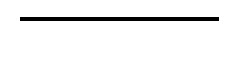
\includegraphics[width=3cm]{Figures/table/use-case/3}}
		& \setstretch{1.5} {เส้นตรงที่แสดงถึงการใช้งาน Use case ของผู้กระทำ} \\ \hline
		\raisebox{-\totalheight}{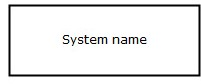
\includegraphics[width=0.3\textwidth]{Figures/table/use-case/4}}
		& \setstretch{1.5} {กรอบสี่เหลี่ยมแสดงถึงขอบเขตของระบบโดยแสดงชื่อระบบภายในหรือด้านบนกรอกสี่เหลี่ยม Use case อยู่ภายในกรอบสี่เหลี่ยม และ actor อยู่ภายนอกกรอบสี่เหลี่ยม} \\ \hline
		\raisebox{-\totalheight}{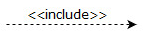
\includegraphics[width=0.3\textwidth]{Figures/table/use-case/5}}
		& \setstretch{1.5} {ความสัมพันธ์แบบ <<includes>> แสดงว่า Use case หนึ่งดำเนินการตามขั้นตอนของ Use case อื่น โดยแทนด้วยสัณลักษณ์ลูกศรเส้นประ ซึ่ง Use case ที่หางลูกศรเรียกใช้งาน Use case ที่หัวลูกศรทุกครั้งที่มีการทำงาน} \\ \hline
		\raisebox{-\totalheight}{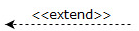
\includegraphics[width=0.3\textwidth]{Figures/table/use-case/6}}
		& \setstretch{1.5} {ความสัมพันธ์แบบ <<extend>> แสดงว่า Use case หนึ่งดำเนินการตามขั้นตอนของ Use case อื่น โดยแทนด้วยสัญลักษณ์ลูกศรเส้นประ ซึ่ง Use case ที่หัวลูกศรเรียกใช้งาน Use case ที่หางลูกศร แต่การใช้งานไม่จำเป็นต้องเกิดขึ้นทุกครั้งขึ้นอยู่กับเงื่อนไขระหว่างการทำงาน} \\ \hline
		\end{tabular}
	\end{table}

	\begin{figure}[H]
		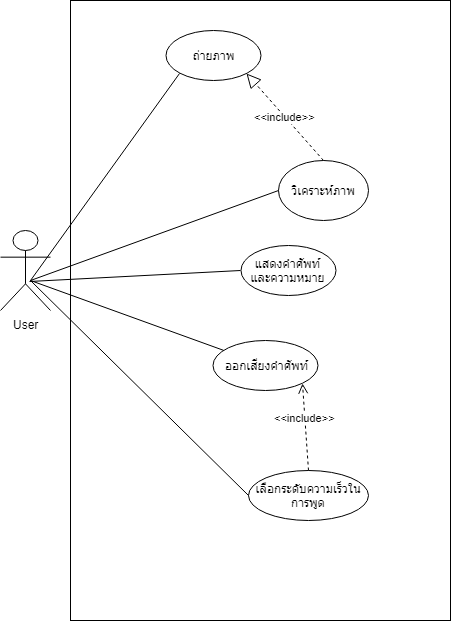
\includegraphics[width=0.9\textwidth]{Figures/3/usecase/usecase.png}
		\caption{Use Case Diagram ของแอปพลิเคชัน What is that}
		\label{Fig:usecase}
	\end{figure}
	
	\begin{table}[H]
		\centering
		\caption{อธิบาย Use Case หน้าที่ของระบบโดยทุกการทำงานจะต้องอาศัยการเข้าสู่ระบบทุกครั้ง ในภาพที่ \ref{Fig:usecase}}
		\label{tab:usecase}
		\resizebox{\totalheight}{!}{\textwidth}{%
			\begin{tabular}{|c|p{8cm}|}
				\hline
				\multicolumn{1}{|c|}{\textbf{Use Case}} & \multicolumn{1}{c|}{\textbf{คำอธิบาย}} \\ \hline
				สแกนอาหาร & สมาชิกสามารถสแกนอาหารแต่ไม่จำเป็นต้องบันทึกข้อมูลการบริโภคทุกครั้ง \\ \hline
				บันทึกแคลลอรี่ น้ำตาล โซเดียมและไขมัน &  การบันทึกข้อมูลการบริโภคสมาชิกไม่จำต้องทำการสแกนทุกครั้ง \\ \hline
				เข้าสู่ระบบ & สมาชิกสามารถทำการเข้าสู่ระบบได้ \\ \hline
				ออกจากระบบ & สมาชิกจะต้องทำการเข้าสู่ระบบก่อนจึงจะสามารถออกจากระบบได้ \\ \hline
				ดูข้อมูลการบริโภครูปแบบวัน สัปดาห์และเดือน & หลังจากสมาชิกทำการเข้าสู่ระบบแล้วสมาชิกสามารถดูข้อมูลการบริโภคในรูปแบบวัน
				 สัปดาห์และเดือนได้  \\ \hline
				ลบอาหารที่เพิ่ม &  สมาชิกสามารถลบอาหารที่เพิ่มเข้ามาได้ด้วยการเลือกที่รายการอาหาร \\ \hline
				เพิ่มอาหารที่ไม่มีในระบบ &  สมาชิกสามารถเพิ่มอาหารที่ไม่มีในระบบเองได้   \\ \hline
			\end{tabular}%
		}
	\end{table}
	% Please add the following required packages to your document preamble:
	% \usepackage{graphicx}
	\begin{table}[H]
		\centering
		\caption{Use Case สแกนอาหาร}
		\label{tab:usecase}
		\resizebox{\totalheight}{!}{\textwidth}{%
			\begin{tabular}{|p{10cm}|p{10cm}|}
				\hline
				\multicolumn{1}{|c|}{\textbf{Use Case Title : สแกนอาหาร}} & \multicolumn{1}{c|}{\textbf{Use case Id : 1 }} \\ \hline
				\multicolumn{2}{|p{\linewidth}|}{Primary Actor : สมาชิก} \\ \hline
			    \multicolumn{2}{|p{\linewidth}|}{Main Flow : สมาชิกจะต้องทำการเข้าสู่ระบบก่อนจึงจะสามารถทำการสแกนได้} \\ \hline
			    \multicolumn{2}{|p{\linewidth}|}{Exceptional Flow ที่ 1 : หากผู้ใช้ไม่เชื่อมต่ออินเทอร์เน็ต จะไม่สามารถทำการสแกนได้} \\ \hline
			\end{tabular}%
		}
	\end{table}
	\begin{table}[H]
		\centering
		\caption{Use Case บันทึกแคลลอรี่ น้ําตาล โซเดียมและไขมัน}
		\label{tab:usecase}
		\resizebox{\totalheight}{!}{\columnwidth}{%
			\begin{tabular}{|p{7cm}|p{7cm}|}
				\hline
				\multicolumn{1}{|c|}{\textbf{Use Case Title : บันทึกแคลลอรี่ น้ําตาล โซเดียมและไขมัน}} & \textbf{Use case Id : 2 } \\ \hline
				\multicolumn{2}{|l|}{Primary Actor : สมาชิก} \\ \hline
				\multicolumn{2}{|p{\linewidth}|}{Main Flow : หากสมาชิกต้องการบันทึกสมาชิกสามารทำการสแกนหรือบันทึกจากอาหารที่เพิ่มเองได้  } \\ \hline
				\multicolumn{2}{|p{\linewidth}|}{Exceptional Flow ที่ 1 : หากสมาชิกไม่เชื่อมต่ออินเทอร์เน็ต จะไม่สามารถทำการบันทึกข้อมูลอาหารได้} \\ \hline
			\end{tabular}%
		}
	\end{table}

	\begin{table}[H]
		\centering
		\caption{Use Case เข้าสู่ระบบ}
		\label{tab:usecase}
		\resizebox{\totalheight}{!}{\textwidth}{%
			\begin{tabular}{|p{7cm}|p{7cm}|}
				\hline
				\multicolumn{1}{|c|}{\textbf{Use Case Title : ดาวน์โหลดเอกสาร}} & \textbf{Use case Id : 3 } \\ \hline
				\multicolumn{2}{|l|}{Primary Actor : สมาชิก} \\ \hline
				\multicolumn{2}{|p{\linewidth}|}{Main Flow : สมาชิกต้องทำการสมัครสมาชิกก่อนจึงจะสามารถทำการเข้าสู่ระบบได้				} \\ \hline
				\multicolumn{2}{|p{\linewidth}|}{Exceptional Flow ที่ 1 : หากสมาชิกไม่เชื่อมต่ออินเทอร์เน็ต จะไม่สามารถทำการเข้าสู่ระบบได้} \\ \hline
				\multicolumn{2}{|p{\linewidth}|}{Exceptional Flow ที่ 2 : หากสมาชิกไม่ทำการสมัครสมาชิกจะไม่สามารถทำการเข้าสู่ระบบได้ } \\ \hline
			\end{tabular}%
		}
		\end{table}
		
		\begin{table}[H]
			\centering
			\caption{Use Case ออกจากระบบ}
			\label{tab:usecase}
			\resizebox{\totalheight}{!}{\textwidth}{%
				\begin{tabular}{|p{10cm}|p{10cm}|}
					\hline
					\multicolumn{1}{|c|}{\textbf{Use Case Title : ออกจากระบบ}} & \multicolumn{1}{c|}{\textbf{Use case Id : 4 }} \\ \hline
					\multicolumn{2}{|l|}{Primary Actor : สมาชิก} \\ \hline
					\multicolumn{2}{|p{\linewidth}|}{Main Flow : สมาชิกจะต้องทำการเข้าสู่ระบบก่อนจึงจะสามารถออกจากระบบได้ } \\ \hline
					\multicolumn{2}{|p{\linewidth}|}{Exceptional Flow ที่ 1 : หากผู้ใช้ไม่ทำการเข้าสู่ระบบ จะไม่สามารถออกจากระบบได้ } \\ \hline
				\end{tabular}%
			}
		\end{table}
		
		\begin{table}[H]
			\centering
			\caption{Use Case ดูข้อมูลการบริโภครูปแบบวัน สัปดาห์และเดือน}
			\label{tab:usecase}
			\resizebox{\totalheight}{!}{\textwidth}{%
				\begin{tabular}{|c|p{10cm}|}
					\hline
					\multicolumn{1}{|c|}{\textbf{Use Case Title : ดูข้อมูลการบริโภครูปแบบวัน สัปดาห์และเดือน}} & \multicolumn{1}{c|}{\textbf{Use case Id : 5 }} \\ \hline
					\multicolumn{2}{|l|}{Primary Actor : สมาชิก} \\ \hline
					\multicolumn{2}{|p{\linewidth}|}{Main Flow : เมื่อสมาชิกทำการเข้าสู่ระบบแล้ว สมาชิกสามารถดูข้อมูลการบริโภคในรูปแบบวัน สัปดาห์และเดือนได้ } \\ \hline
					\multicolumn{2}{|p{\linewidth}|}{Exceptional Flow ที่ 1 : หากผู้ใช้ไม่เชื่อมต่ออินเทอร์เน็ต จะไม่สามารถดูข้อมูลการบริโภคในรูปแบบวัน สัปดาห์และเดือนได้} \\ \hline
				\end{tabular}%
			}
		\end{table}
	
		\begin{table}[H]
			\centering
			\caption{Use Case ลบอาหารที่เพิ่ม}
			\label{tab:usecase}
			\resizebox{\totalheight}{!}{\textwidth}{%
				\begin{tabular}{|c|p{10cm}|}
					\hline
					\multicolumn{1}{|c|}{\textbf{Use Case Title : ลบอาหารที่เพิ่ม}} & \multicolumn{1}{c|}{\textbf{Use case Id : 6 }} \\ \hline
					\multicolumn{2}{|l|}{Primary Actor : สมาชิก} \\ \hline
					\multicolumn{2}{|p{\linewidth}|}{Main Flow :  สมาชิกสามารถทำการลบอาหารได้ด้วยการเลือกที่เมนูอาหาร} \\ \hline
					\multicolumn{2}{|p{\linewidth}|}{Exceptional Flow ที่ 1 : หากสมาชิกไม่เชื่อมต่ออินเทอร์เน็ต จะไม่สามารถทำการลบอาหารได้} \\ \hline
				\end{tabular}%
			}
		\end{table}	
		
		\begin{table}[H]
			\centering
			\caption{Use Case เพิ่มอาหารท่ีไม่มีในระบบ}
			\label{tab:usecase}
			\resizebox{\totalheight}{!}{\textwidth}{%
				\begin{tabular}{|c|p{10cm}|}
					\hline
					\multicolumn{1}{|c|}{\textbf{Use Case Title : เพิ่มอาหารท่ีไม่มีในระบบ}} & \multicolumn{1}{c|}{\textbf{Use case Id : 7 }} \\ \hline
					\multicolumn{2}{|l|}{Primary Actor : สมาชิก} \\ \hline
					\multicolumn{2}{|p{\linewidth}|}{Main Flow :  สมาชิกสามารถเพิ่มอาหารที่ไม่มีในระบบได้ด้วยการกดปุ่ม ADD  } \\ \hline
					\multicolumn{2}{|p{\linewidth}|}{Exceptional Flow ที่ 1 : หากสมาชิกไม่เชื่อมต่ออินเทอร์เน็ต จะไม่สามารถเพิ่มอาหารได้} \\ \hline
				\end{tabular}%
			}
		\end{table}	
%		\begin{table}[H]
%			\centering
%			\caption{Use Case สมัครสมาชิก}
%			\label{tab:usecase}
%			\resizebox{\totalheight}{!}{\textwidth}{%
%				\begin{tabular}{|c|p{10cm}|}
%					\hline
%					\multicolumn{1}{|c|}{\textbf{Use Case Title : สมัครสมาชิก}} & \multicolumn{1}{c|}{\textbf{Use case Id : 8 }} \\ \hline
%					\multicolumn{2}{|l|}{Primary Actor : นักศึกษา} \\ \hline
%					\multicolumn{2}{|l|}{Stakeholder Actor : -} \\ \hline
%					\multicolumn{2}{|p{\linewidth}|}{Main Flow : เมื่อนักศึกษาต้องการใช้งานระบบทั้งหมดของกองทุนจำเป็นต้องเข้าสู่ระบบก่อน หากยังไม่มีบัญชีสามารถสมัครได้โดยต้องกรอกข้อมูลอีเมลและรหัสผ่าน} \\ \hline
%					\multicolumn{2}{|p{\linewidth}|}{Exceptional Flow ที่ 1 : หากผู้ใช้ไม่เชื่อมต่ออินเทอร์เน็ต จะไม่สามารถสมัครสมาชิกได้} \\ \hline
%				\end{tabular}%
%			}
%		\end{table}	
%		 \begin{table}[H]
%		 	\centering
%		 	\caption{Use Case เข้าสู่ระบบ}
%		 	\label{tab:usecase}
%		 	\resizebox{\totalheight}{!}{\textwidth}{%
%		 		\begin{tabular}{|c|p{10cm}|}
%		 			\hline
%		 			\multicolumn{1}{|c|}{\textbf{Use Case Title : เข้าสู่ระบบ}} & \multicolumn{1}{c|}{\textbf{Use case Id : 9 }} \\ \hline
%		 			\multicolumn{2}{|l|}{Primary Actor : นักศึกษา} \\ \hline
%		 			\multicolumn{2}{|l|}{Stakeholder Actor : -} \\ \hline
%		 			\multicolumn{2}{|p{\linewidth}|}{Main Flow : เมื่อนักศึกษาต้องการใช้งานระบบทั้งหมดของกองทุนจำเป็นต้องเข้าสู่ระบบก่อนโดยต้องกรอกข้อมูลอีเมลและรหัสผ่าน} \\ \hline
%		 			\multicolumn{2}{|p{\linewidth}|}{Exceptional Flow ที่ 1 : หากผู้ใช้ไม่เชื่อมต่ออินเทอร์เน็ต จะไม่สามารถเข้าสู่ระบบได้} \\ \hline
%		 		\end{tabular}%
%		 	}
%		 \end{table}	
	
\newpage

\section{Class Diagram}
	Class Diagram คือแผนภาพที่ใช้แสดงคลาสและความสัมพันธ์ในแบบต่างๆ ระหว่างคลาส สัญลักษณ์ที่ใช้ในการเขียน Class Diagram แสดงในตารางที่ \ref{tab:class2} 
	\begin{center}
	\begin{table}[H]
		\centering
		\caption{สัญลักษณ์ของ Class Diagram}
		\label{tab:class2}
		\begin{tabular}{|c|p{10cm}|}
			\hline
			\textbf{สัญลักษณ์} & \multicolumn{1}{c|}{\textbf{การใช้งาน}} \\ \hline
			\raisebox{-\totalheight}{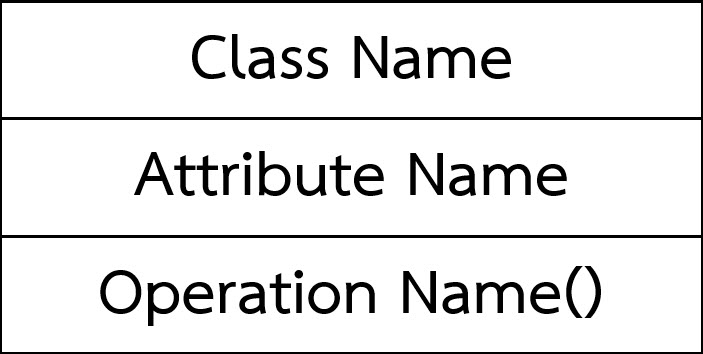
\includegraphics[width=0.3\textwidth]{Figures/table/class/11}}
			& \setstretch{1.5} {คลาส สัญลักษณ์แทนด้วยสี่เหลี่ยมแบ่งเป็น 3 ส่วน 
				ส่วนบน เป็นชื่อของ class ส่วนกลาง เป็นชื่อ Attribute และส่วนล่างเป็น Operation Name หรือ Method ใช้สำหรับเขียนฟังก์ชันในการทำงานของคลาสนั้น ๆ
				ชนิดของ Visibility ของ Method และ Attribute
				แบ่งเป็น 3 ชนิด ได้แก่
				\begin{enumerate}
					\item Public แทนสัญลักษณ์ด้วยเครื่องหมายบวก (+)
					\item Private แทนสัญลักษณ์ด้วยเครื่องหมายลบ (-)
					\item Protected แทนสัญลักษณ์ด้วยเครื่องหมายชาร์ป (#)
				\end{enumerate}
			} \\ \hline
			\raisebox{-\totalheight}{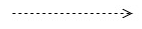
\includegraphics[width=0.3\textwidth]{Figures/table/class/1}}
			& \setstretch{1.5} {Dependency Relationship หมายความว่า คลาสที่อยู่ฝั่งต้นลูกศรสามารถเรียกใช้คลาสที่อยู่ฝั่งหัวลูกศร}
			\\ \hline
			\raisebox{-\totalheight}{
\includegraphics[width=0.35\textwidth]{Figures/3/Class/aggre}}
			& \setstretch{1.5} {Composition Relationship เป็นความสัมพันธ์ระหว่างออบเจ็กต์หรือคลาสแบบขึ้นต่อกันและมีความเกี่ยวข้องกันเสมอ} \\ \hline
			\raisebox{-\totalheight}{
\includegraphics[width=0.3\textwidth]{Figures/3/Class/implement}}
			& \setstretch{1.5} {Realization Relationship เป็นความสัมพันธ์ระหว่าง Object หรือ Class ในลักษณะของการสืบทอดคุณสมบัติจาก Class หนึ่ง (Super class) ไปยังอีก Class หนึ่ง (Subclass)} \\ \hline
			\raisebox{-\totalheight}{
\includegraphics[width=50,height=50]{Figures/table/class/connector}}
			& \setstretch{1.5} {Connector เป็นสัญลักษณ์แทนด้วยรูปห้าเหลี่ยมและมีชื่ออยู่ตรงกลาง จะสร้างสัญลักษณ์นี้ไว้เมื่อต้องการเชื่อมต่อคลาสที่อยู่คนละหน้า} \\ \hline
		\end{tabular}
	\end{table}
	\end{center}

\newpage
	%IMAGE of class

	Class Diagram แสดงความสัมพันธ์ในรูปแบบต่างๆ ระหว่างคลาสของแอปพลิเคชันระบบกองทุนเงินให้กู้ยืมเพื่อการศึกษา คณะวิทยาศาสตร์ มหาวิทยาลัยอุบลราชธานี อธิบายได้ตามภาพที่ \ref{Fig:MainActivity20C} ดังต่อไปนี้
	

	\begin{figure}[H]

		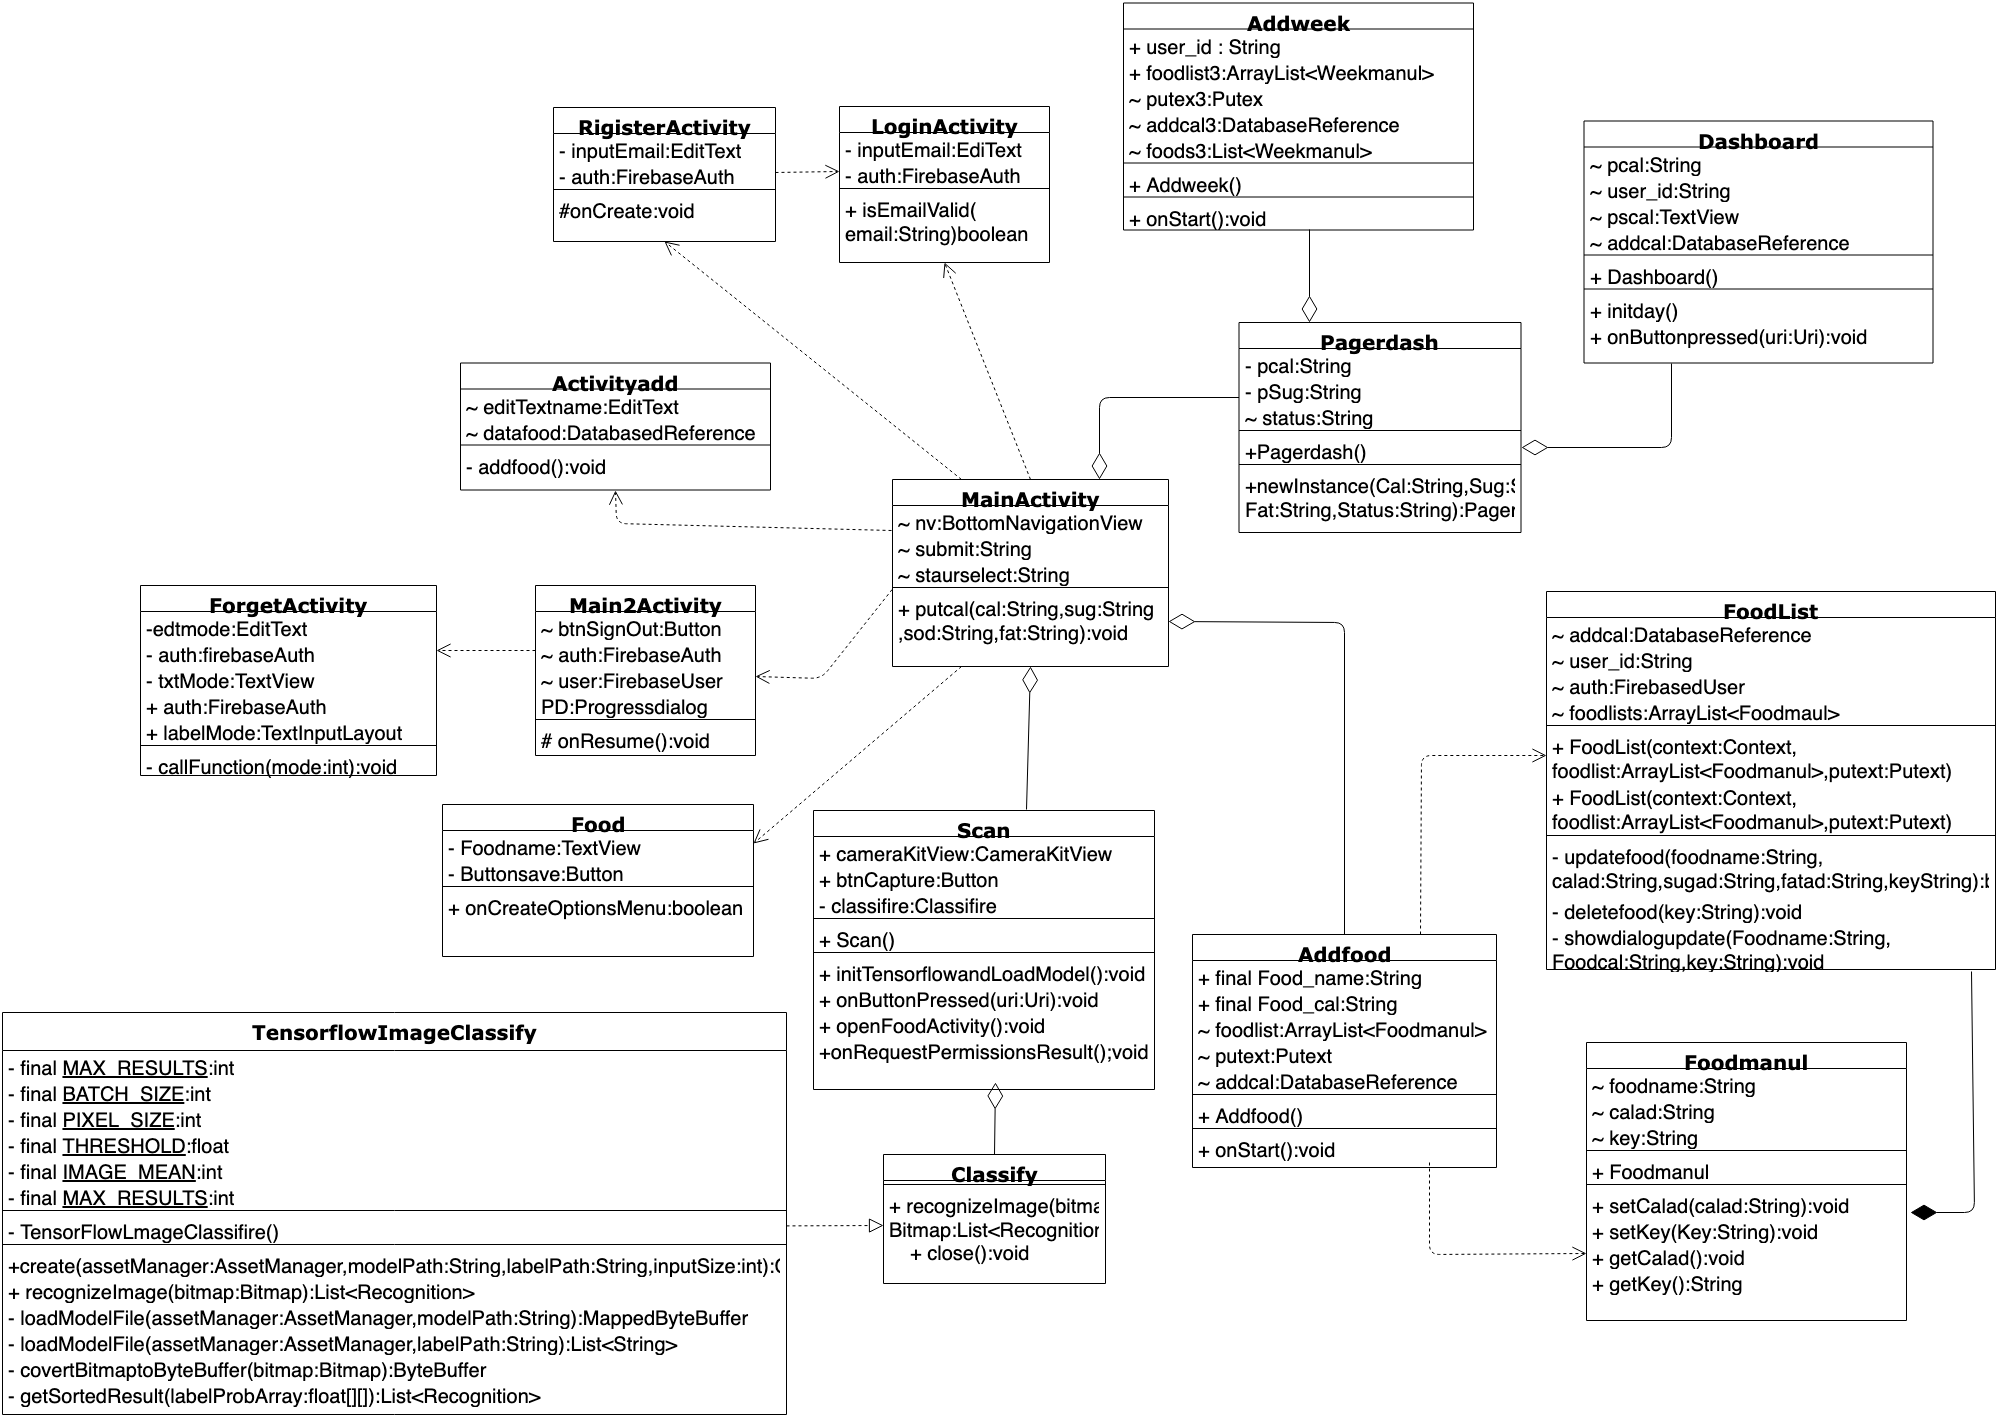
\includegraphics[width=1.1\columnwidth]{Figures/3/Class/class14.png}
		\caption{Class Diagram ของแอปพลิเคชันบีอิงเวลเนส}
		\label{Fig:MainActivity20C}
	\end{figure}


	% TABLE of class
\newpage	
	จากรูปภาพที่ \ref{Fig:MainActivity20C} สามารถอธิบายแผนภาพ Class Diagram ได้ดังนี้
	\begin{table}[H]
		\centering
		\caption{อธิบาย Class Diagram ของแอปพลิเคชันบีอิงเวลเนส}
		\label{tab:class}
		\begin{tabular}{|c|p{10cm}|}
			\hline
			\textbf{Class Diagram} & \multicolumn{1}{c|}{\textbf{คำอธิบาย}} \\ \hline
			\raisebox{-\totalheight}{LoginActivity}
			& \setstretch{1.5} {คลาส LoginActivity จะถูกเรียกใช้เมื่อสมาชิกเปิดแอพพลิเคชัน โดยวัตถุประสงค์การทำงานของคลาสนี้คือ เพื่อให้สมาชิกทำการเข้าสู่ระบบและสมัครสมาชิก } \\ \hline
			\raisebox{-\totalheight}{RigisterActivity}
			& \setstretch{1.5} {คลาส RigisterActivity จะถูกใช้งานเมื่อผู้ใช้กดปุ่ม SiGN UP โดยวัตถุประสงค์การทำงานของคลาสคือ เพื่อให้สมาชิกทำการสมัครสมาชิก} \\ \hline
			\raisebox{-\totalheight}{MainActivity}
			& \setstretch{1.5} {คลาส MainActivity เป็นคลาสหลักที่ใช้ในการทำงานของแอปพลิเคชันโดยการทำงานของคลาสนี้เน้นไปที่การเรียกใช้ Fragment โดยองค์ประกอบของคลาสนี้ประกอบไปด้วยคลาสของ Fragment ได้แก่ Pagerdash Myfood Scan} \\ \hline
			\raisebox{-\totalheight}{Main2Activiy}
			& \setstretch{1.5} {คลาส Main2Activiy เป็นคลาสที่ให้สมาชิกได้เลือกการจัดการบัญชีสมาชิก ได้แก่ เปลี่ยนอีเมล เปลี่ยนรหัสผ่าน ลบผู้ใช้ และออกจากระบบ} \\ \hline
			\raisebox{-\totalheight}{ForgetActivity}
			& \setstretch{1.5} {คลาส ForgetActivity  เป็นคลาสที่ทำการจัดการบัญชีสมาชิก ได้แก่ เปลี่ยนอีเมล เปลี่ยนรหัสผ่าน ลบผู้ใช้  } \\ \hline
			\raisebox{-\totalheight}{Activityadd}
			& \setstretch{1.5} {คลาส Activityadd  เป็นคลาสที่มีไว้สำหรับให้สมาชิกเพิ่มอาหารที่ไม่มีในระบบ } \\ \hline
			\raisebox{-\totalheight}{Food}
			& \setstretch{1.5} {คลาส Food  จะถูกใช้งานเมื่อสมาชิกทำการสแกนอาหาร โดยวัตถุประสงค์การทำงานของคลาสคือเพื่อแสดงข้อมูลอาหารที่สแกนได้ } \\ \hline

	\end{tabular}
\end{table}

\newpage
\begin{table}[H]
	\centering
	\caption{อธิบาย Class Diagram ของแอปพลิเคชันบีอิงเวลเนส(ต่อ)}
	\label{tab:class}
	\begin{tabular}{|c|p{10cm}|}
		\hline
		\textbf{Class Diagram} & \multicolumn{1}{c|}{\textbf{คำอธิบาย}} \\ \hline
		\raisebox{-\totalheight}{Pagerdash}
		& \setstretch{1.5} {คลาส Pagerdash เป็นคลาสหลักที่ใช้ในการจัดการ Tab เมนูในการเลื่อนเพื่อดูรูปแบบของข้อมูลการบริโภค} \\ \hline
		\raisebox{-\totalheight}{Addweek}
		& \setstretch{1.5} {คลาส Addweek  เป็นคลาสที่จะแสดงเมื่อสมาชิกทำการเลื่อนมาที่ Tab Week เป็นคลาสที่แสดงข้อมูลการบริโภคในรูปแบบสัปดาห์} \\ \hline
		\raisebox{-\totalheight}{Dashboard}
		& \setstretch{1.5} {คลาส Dashboard เป็นคลาสหลักที่จะถูกเรียกใช้เมื่อผู้ใช้ทำการเปิดแอปพลิเคชันหลังจากทำการเข้าสู่ระบบแล้ว โดยวัตถุประสงค์การทำงานของคลาสนี้คือ แสดงข้อมูลการบริโภคในรูปแบบวัน} \\ \hline
		\raisebox{-\totalheight}{Addfood}
		& \setstretch{1.5} {คลาส Addfood เป็นคลาสที่จะแสดงเมื่อผู้ใช้เลือกเมนู My food โดยวัตถุประสงค์การทำงานของคลาสคือแสดงรายการอาหารที่เพิ่มเข้ามา} \\ \hline
		\raisebox{-\totalheight}{FoodList}
		& \setstretch{1.5} {คลาส FoodList เป็นคลาสที่จะถูกใช้งานเมื่อคลาส Addfood ถูกใช้ โดยวัตถุประสงค์การทำงานของคลาสคือ จัดรูปแบบการแสดงรายการอาหาร} \\ \hline
		\raisebox{-\totalheight}{Foodmanul}
		& \setstretch{1.5} {คลาส Foodmanul เป็นคลาสที่กำหนดค่าต่างๆที่จำเป็นในการสร้างรายการอาหาร} \\ \hline
		\raisebox{-\totalheight}{Scan}
		& \setstretch{1.5} {คลาส Scan เป็นคลาสที่จะแสดงเมื่อผู้ใช้เลือกเมนู Scan โดยวัตถุประสงค์การทำงานของคลาสคือสแกนอาหาร} \\ \hline
		\raisebox{-\totalheight}{Classify}
		& \setstretch{1.5} {คลาส Classify เป็นคลาสที่ทำงานหลังจากสมาชิกทำการสแกน โดยวัตถุประสงค์การทำงานของคลาสคือแยกประเภทรูปภาพที่สมาชิกทำการถ่าย} \\ \hline
		\raisebox{-\totalheight}{TensorflowImageClassify}
		& \setstretch{1.5} {คลาส TensorflowImageClassify เป็นคลาสที่ทำงานร่วมกับคลาส  Classify โดยจะทำหน้าที่นำโมเดลเข้ามาเพื่อใช้ในการระบุภาพอาหารที่สมาชิกทำการถ่าย } \\ \hline
	\end{tabular}
\end{table}

\newpage
\section{Sequence Diagram}
	Sequence Diagram เป็น Diagram ที่แสดงขั้นตอนการทำงานของแต่ละ Use Case ระหว่าง Object ต่างๆ  โดย Sequence Diagram จะช่วยให้มองเห็นการทำงานของภาพรวมของระบบ ส่วนประกอบสัญลักษณ์ที่ใช้ในการเขียน Sequence Diagram 
	แสดงดังตารางที่ \ref{tab:Sequences}
	
	\begin{table}[H]
		\centering
		\caption{สัญลักษณ์ของ Sequence Diagram}
		\label{tab:Sequences}
		\begin{tabular}{| c	| p{10cm} |}
		\hline
		\textbf{สัญลักษณ์} & \multicolumn{1}{c|}{\textbf{การใช้งาน}} \\ \hline
		\raisebox{-\totalheight}{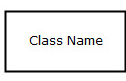
\includegraphics[width=0.17\textwidth]{Figures/table/Sequence/Sequence1}}
		& \setstretch{1.5} {Class แสดงถึงการทำงานของ Use Case ในการส่งหรือรับข้อความ แทนด้วยสัญลักษณ์สี่เหลี่ยมมีชื่อคลาสอยู่ภายใน} \\ \hline
		\raisebox{-\totalheight}{
\includegraphics[height=0.08\textheight]{Figures/table/Sequence/Sequence2}}
		& \setstretch{1.5} {Lifeline หรือเส้นอายุขัย แสดงช่วงเวลาตั้งแต่เริ่มสร้าง object ในคลาสนั้น จนกระทั่ง object นั้นถูกทำลาย สัญลักษณ์แทนด้วยเส้นประ} \\ \hline
		\raisebox{-\totalheight}{
\includegraphics[height=0.08\textheight]{Figures/table/Sequence/Sequence3}}
		& \setstretch{1.5} {Focus of control หรือจุดควบคุม เป็นจุดควบคุมที่ object ใช้ทำการส่งหรือรับข้อความ สัญลักษณ์แทนด้วยสี่เหลี่ยม} \\ \hline
		\raisebox{-\totalheight}{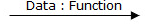
\includegraphics[width=0.3\textwidth]{Figures/table/Sequence/Sequence4}}
		& \setstretch{1.5} {Message คือ ข้อความที่รับส่งระหว่าง Object สัญลักษณ์แทนด้วยลูกศรและประกอบด้วย 2 ส่วน คือ ข้อมูล (Data) และฟังก์ชัน (Function)} \\ \hline
		\raisebox{-\totalheight}{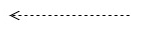
\includegraphics[width=0.3\textwidth]{Figures/table/Sequence/Sequence5}}
		& \setstretch{1.5} {Return Message เป็นข้อมูลที่ส่งกลับหลังจากทำงานเสร็จ} \\ \hline
		\raisebox{-\totalheight}{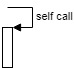
\includegraphics[height=0.08\textheight]{Figures/3/selfcall}}
		& \setstretch{1.5} {Self call เป็นการเรียกฟังชันก์การทำงานภายในตัวเอง} \\ \hline
		\raisebox{-\totalheight}{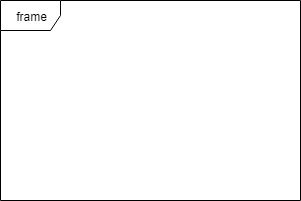
\includegraphics[height=0.1\textheight,width=0.3\textwidth]{Figures/3/frame}}
		& \setstretch{1.5} {สร้างกรอบการทำงานของโปรแกรม เพื่อให้รู้ขอบเขตของการทำงานเช่น ลูป(loop)} \\ \hline
		\end{tabular}
	\end{table}
%
%	Sequence Diagram ที่ใช้อธิบายการทำงานของระบบกองทุนเงินให้กู้ยืมเพื่อการศึกษา คณะวิทยสศาสตร์ มหาวิทยาลัยอุบลราชธานี มีรายละเอียดดังต่อไปนี้

\newpage
	\begin{landscape}
	\begin{figure}[H]
		\centering
		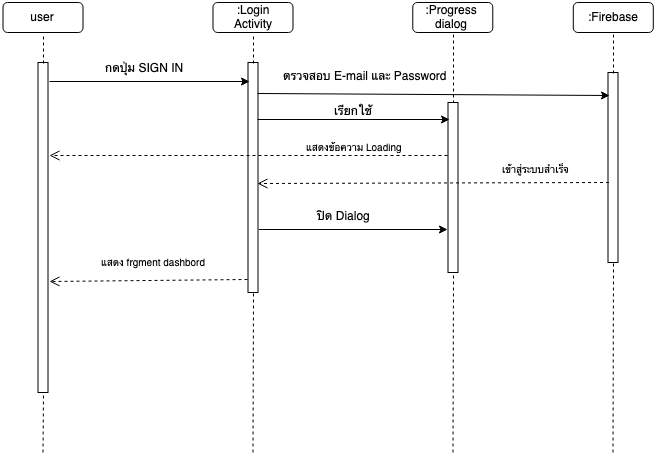
\includegraphics[width=0.8\columnwidth]
		{Figures/3/Sequence/sqlogin.png}
		\caption{Sequence Diagram การเข้าสู่ระบบ}
		\label{Fig:Sequence-login}
	\end{figure}
  \end{landscape}

		\label{Fig:Sequence-login}
		จากภาพที่ \ref{Fig:Sequence-login} สามารถอธิบายแผนภาพ Sequence Diagram การเข้าสู่ระบบ ได้ดังนี้ เมื่อ
	สมาชิกกดปุ่ม SIGN IN  ที่คลาส LoginActivity จะทำการตรวจสอบ E-mail และ Password โดยส่งไปที่ Firebase ในขณะเดียวกันก็จะเรียก Progess dialog แสดงข้อความไปยังสมาชิกว่า Loading 
	 เมื่อเข้าสู่ระบบสำเร็จจะทำการปิด Dialog แล้วแสดง fragment dashbord ที่สมาชิก
	\begin{sidewaysfigure}
	\begin{figure}[H]
		\centering
		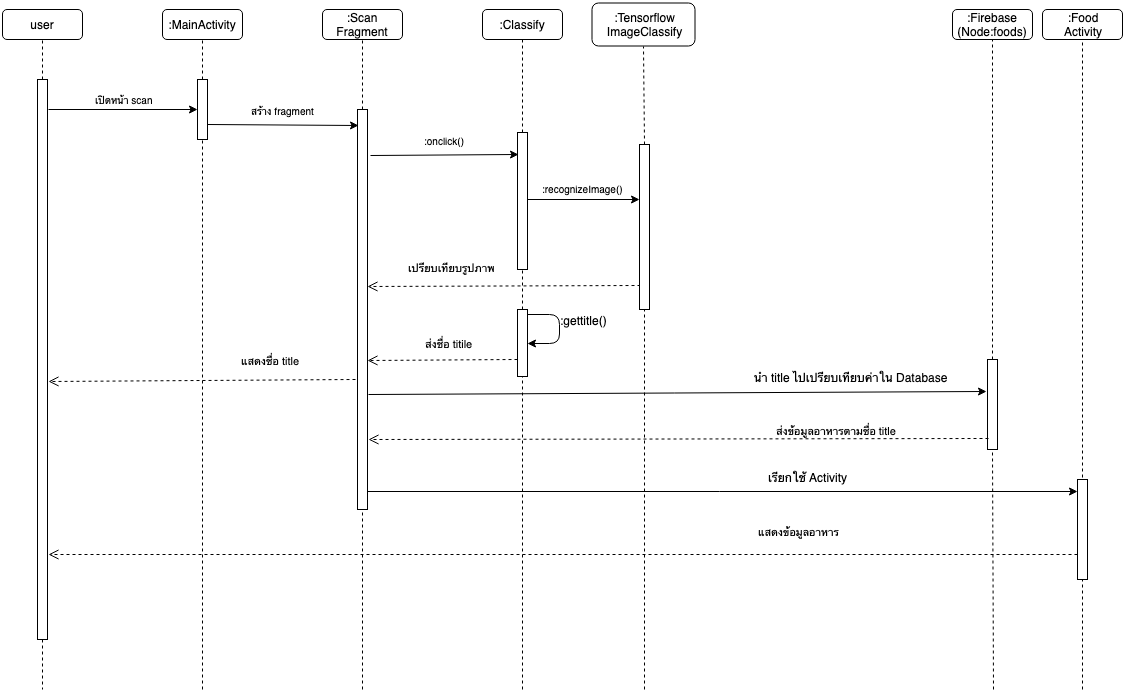
\includegraphics[width=0.8\columnwidth]
		{Figures/3/Sequence/sqscannew1.png}
		\caption{Sequence Diagram การสแกน}
		\label{Fig:Sequence-scan}
	\end{figure}
	\end{sidewaysfigure}
	\newpage
	จากภาพที่ \ref{Fig:Sequence-scan} สามารถอธิบายแผนภาพ Sequence Diagram การสแกน ได้ดังนี้ เมื่อสมาชิกทำการเปิดหน้าสแกน คลาส MainActivity จะทำการสร้่าง Fragent Scan ขึ้นมาและเมื่อสมาชิกกดปุ่ม Scan ฟังก์ชัน Onclick() จะทำการส่งข้อมูลไปยังคลาส Classify จากนั้นคลาส Classify 
	จะทำการ :recognizeImage() แล้วให้คลาส TensorflowImageClassify ทำการเปรียบเทียบรูปภาพ หลังจากการเปรียบเทียบรูปภาพแล้วที่ Fragment Scan จะใช้เมธอด getitile() แล้วส่งชื่อ title ที่ได้มาแสดงให้หับสมาชิก แล้วนำ title ที่แสดงไปเปรียบกับค่าใน Firebased ที่โหนด foods แล้วส่งข้อมูลหารที่ตรงกันกับ title 
	จากนั้นเรียกใช้ FoodActivity ที่หแสดงข้อมูลอาหารให้กับสมาชิก
 
	\begin{sidewaysfigure}
	\begin{figure}[H]
		\centering
		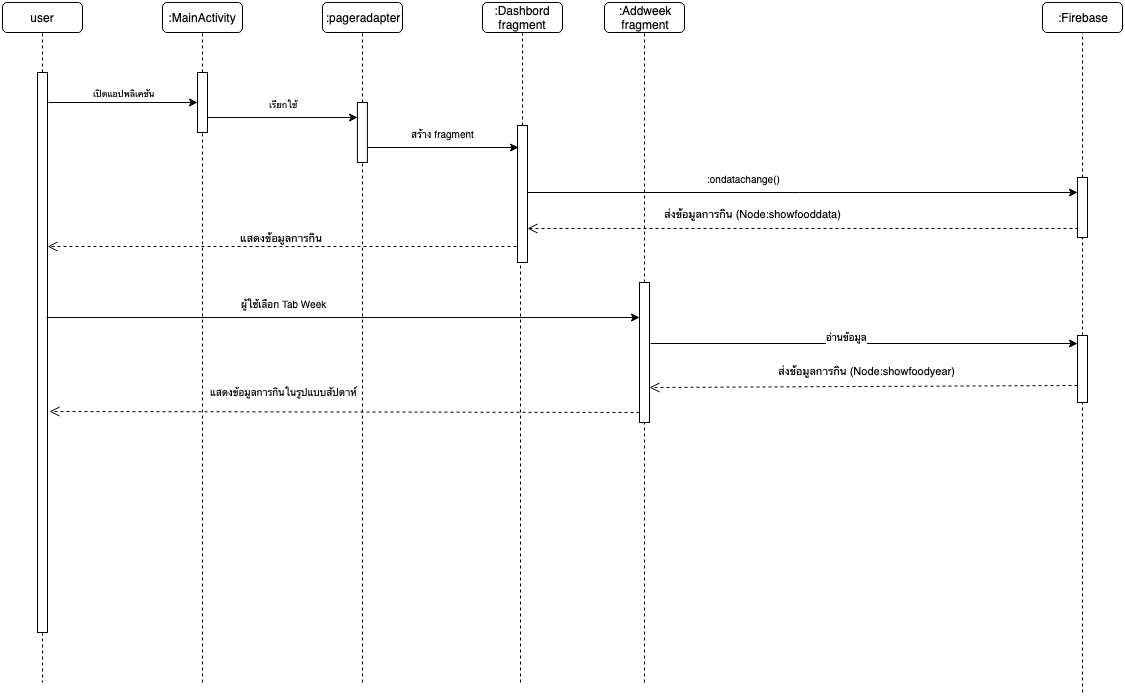
\includegraphics[width=1\columnwidth]
		{Figures/3/Sequence/sqtabnew.png}
		\caption{Sequence Diagram ดูข้อมูลการบริโภครูปแบบวัน สัปดาห์และเดือน}
		\label{Fig:Sequence-sqtab}
	\end{figure}
	\end{sidewaysfigure}
	\newpage
	จากภาพที่ \ref{Fig:Sequence-sqtab} สามารถอธิบายแผนภาพ Sequence Diagram ดูข้อมูลการบริโภครูปแบบวัน สัปดาห์และเดือน ได้ดังนี้ เมื่อสมาชิกเปิดแอปพลิเคชันคลาส MainActivity จะเรียกใช้ Pagerdash  
	ซึ่งประกอบไปด้วย Fragment ดังนี้  Dashboard Addweek และ Addmonth 	จากนั้นแต่ละ Fragment จะทำเมธอด ondatachange() 
	ด้วยการอ่านข้อมูลที่ Firebase โหนด Showfooddata Showfoodyear และ ShowfoodMonth ตาม Tab ที่ผู้ใช้เลือกดู

	\begin{sidewaysfigure}
	\begin{figure}[H]
		\centering
		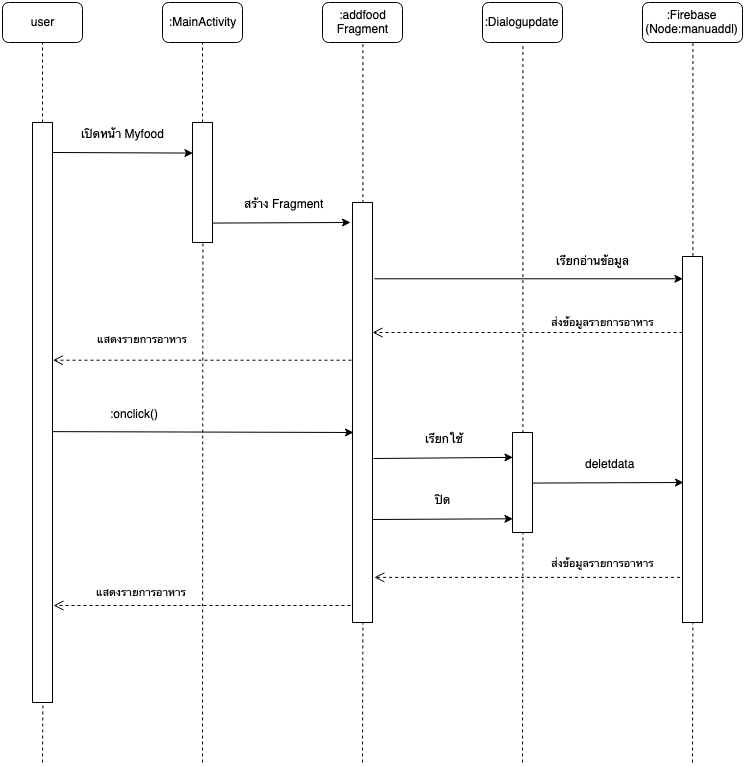
\includegraphics[width=0.6\columnwidth]
		{Figures/3/Sequence/sqdelete.png}
		\caption{Sequence Diagram ลบอาหารที่เพิ่ม}
		\label{Fig:Sequence-delete}
	\end{figure}
	\end{sidewaysfigure}
	\newpage
	จากภาพที่ \ref{Fig:Sequence-delete} สามารถอธิบายแผนภาพ Sequence Diagram ลบอาหารที่เพิ่ม ได้ดังนี้ เมื่อผู้ใช้เปิดหน้า Myfood คลาส MainActivity จะทำการสร้าง Fragment addfood  จากนั้นจะทำการอ่านข้อมูลที่ Firebase มาแสดงรายการอาหารที่สมาชิก และเมื่อผู้ใช้กดที่รายการอาหาร  Fragment addfood  จะเรียกใช้ Dialogupdate แล้วลบข้อมูลออก หลังจากที่ลบข้อมูลแล้วก็จะทำการปิด Dialogupdate 
	จากนั้น Firebase จะส่งข้อมูลรายการอาหารที่มีอยู่มา แสดงที่สมาชิกอีกครั้ง
	\newpage	

	
\section{โครงสร้างฐานข้อมูลไฟร์เบส(Firebase Database Stucture)}
Firebase Database นั้นเป็น Database แบบ NoSQL และเป็น JSON database ที่มีโครงสร้างที่เป็น Key และ Value จัดเก็บข้อมูลในลักษณะโหนด หากต้องการเรียกงานจะเรียกใช้โดย
การท่องไปยังโหนดที่ต้องการ ส่วนประกอบสัญลักษณ์ที่ใช้ในการเขียนโครงสร้างฐานข้อมูลแบบ Firebase
แสดงดังตารางที่ \ref{tab:DB}

\begin{table}[H]
	\centering
	\caption{สัญลักษณ์ของโครงสร้างฐานข้อมูลแบบ Firebase}
	\label{tab:DB}
	\begin{tabular}{| c	| p{10cm} |}
		\hline
		\textbf{สัญลักษณ์} & \multicolumn{1}{c|}{\textbf{คำอธิบาย}} \\ \hline
		\raisebox{-\totalheight}{
\includegraphics[width=0.1\textwidth]{Figures/3/DB/dbroot}}
		& \setstretch{1.5} {Database เป็นการเรียกชื่อแทนรูทโหนด(Root Node)บนสุดที่ใช้ในการเก็บข้อมูล} \\ \hline
		\raisebox{-\totalheight}{
\includegraphics[width=0.1\textwidth]{Figures/3/DB/dbcollection}}
		& \setstretch{1.5} {Key  เป็นโหนด(Node) ที่รองลงมาจากรูทโหนด ซึ่งประกอบไปด้วย KeyและValue } \\ \hline
	\end{tabular}
\end{table}
	\begin{figure}[H]
	\centering
	
\includegraphics[width=0.7\columnwidth]
	{Figures/3/DB/firebase.png}
	\caption{โครงสร้างฐานข้อมูลแบบ Firebase}
	\label{Fig:DB1}
	\end{figure}

	\begin{figure}[H]
	\centering
	
\includegraphics[width=0.6\columnwidth]
	{Figures/3/DB/firebase2.png}
	\caption{โครงสร้างฐานข้อมูลแบบ Firebase(ต่อ)}
	\label{Fig:DB2}
\end{figure}
	\begin{figure}[H]
	\centering
	
\includegraphics[width=0.7\columnwidth]
	{Figures/3/DB/showfoodmonth.png}
	\caption{โครงสร้างฐานข้อมูลแบบ Firebase(ต่อ)}
	\label{Fig:DB3}
\end{figure}
	

\newpage
จากรูที่ \ref{Fig:DB1}-\ref{Fig:DB3} สามารถอธิบายโครงสร้างของข้อมูลได้ดังนี้
\begin{figure}[H]
\centering

\includegraphics[width=0.6\columnwidth]
{Figures/3/DB/nodefood.png}
\caption{โหนดเก็บข้อมูลประกาศ}
\label{Fig:DB4}
\end{figure}
\begin{table}[H]
	\centering
	\caption{อธิบายโหนดที่ใช้เก็บข้อมูลอาหาร}
	\label{my-label1}
	\begin{tabular}{|c|p{10cm}|}
		\hline
		\multicolumn{1}{|c|}{\textbf{Key}} & \multicolumn{1}{c|}{\textbf{คำอธิบาย}} \\ \hline
		foods & โหนดสำหรับเก็บข้อมูลอาหารในระบบทั้งหมก \\ \hline
		Key &  โหนดสำหรับเก็บคีย์ของอาหาร \\ \hline
		Calories & สำหรับเก็บแคลลอรี่ของอาหาร \\ \hline
		Fat & สำหรับเก็บค่าไขมันของอาหาร  \\ \hline
		Name &  สำหรับเก็บชื่อของอาหาร \\ \hline
		Sodium &  สำหรับเก็บค่าโซเดียมของอาหาร \\ \hline
		Sugar & สำหรับเก็บค่าน้ำตาลของอาหาร \\ \hline
		\end{tabular}
\end{table}

\newpage
\begin{figure}[H]
	\centering
	
\includegraphics[width=0.7\columnwidth]
	{Figures/3/DB/manuladd.png}
	\caption{โหนดเก็บข้อมูลอาหารที่สมาชิกเพิ่มเข้ามา}
	\label{Fig:DB4}
\end{figure}
\begin{table}[H]
	\centering
	\caption{อธิบายโหนดเก็บข้อมูลอาหารที่สมาชิกเพิ่มเข้ามา}
	\label{my-label1}
	\begin{tabular}{|c|p{10cm}|}
		\hline
		\multicolumn{1}{|c|}{\textbf{Key}} & \multicolumn{1}{c|}{\textbf{คำอธิบาย}} \\ \hline
		manuladd & โหนดสำหรับเก็บข้อมูลอาหารที่สมาชิกเพิ่มเข้ามาทั้งหมด \\ \hline
		user\_id &  โหนดสำหรับเก็บข้อมูลอาหารที่เพิ่มเข้าของสมาชิกแต่ละคน\\ \hline
		key & โหนดสำหรับเก็บ ID ของอาหารที่สมาชิกเพิ่มเข้ามา \\ \hline
		calad & สำหรับเก็บแคลลอรี่ของอาหารที่ผู้ใช้เพิ่มเข้ามา \\ \hline
		fatad & สำหรับเก็บแคลลอรี่ของอาหารที่ผู้ใช้เพิ่มเข้ามา\\ \hline
		foodname & สำหรับเก็บแคลลอรี่ของอาหารที่ผู้ใช้เพิ่มเข้ามา\\ \hline
		sodad & สำหรับเก็บแคลลอรี่ของอาหารที่ผู้ใช้เพิ่มเข้ามา\\ \hline
		sugad & สำหรับเก็บแคลลอรี่ของอาหารที่ผู้ใช้เพิ่มเข้ามา\\ \hline

	\end{tabular}
\end{table}

\newpage
\begin{figure}[H]
	\centering
	
\includegraphics[width=0.6\columnwidth]
	{Figures/3/DB/showfooddata.png}
	\caption{โหนดเก็บข้อมูลการบริโภคในรูปแบบวัน}
	\label{Fig:DB4}
\end{figure}
\begin{table}[H]
	\centering
	\caption{อธิบายโหนดเก็บข้อมูลการบริโภคในรูปแบบวัน}
	\label{my-label1}
	\begin{tabular}{|c|p{10cm}|}
		\hline
		\multicolumn{1}{|c|}{\textbf{Key}} & \multicolumn{1}{c|}{\textbf{คำอธิบาย}} \\ \hline
		showfooddata & โหนดสำหรับเก็บข้อมูลการบริโภคในรูปแบบวันทั้งหมด\\ \hline
		User\_id &  สำหรับเก็บข้อมูลการบริโภคในรูปแบบวันของสมาชิกแต่ละคน \\ \hline
		Key & สำหรับเก็บข้อมูลวันที่ \\ \hline
		totalcal & สำหรับเก็บข้อมูลแคลลอรี่ในรูปแบบวัน \\ \hline
		totalfat & สำหรับเก็บข้อมูลไขมันรี่ในรูปแบบวัน \\ \hline
		totalsod & สำหรับเก็บข้อมูลโซเดียมในรูปแบบวัน\\ \hline
		totalsug & สำหรับเก็บข้อมูลน้ำตาลในรูปแบบวัน\\ \hline
	
	\end{tabular}
\end{table}

\newpage
\begin{figure}[H]
	\centering
	
\includegraphics[width=0.6\columnwidth]
	{Figures/3/DB/showfoodyear.png}
	\caption{โหนดเก็บข้อมูลการบริโภคในรูปแบบสัปดาห์}
	\label{Fig:DB4}
\end{figure}
\begin{table}[H]
	\centering
	\caption{อธิบายโหนดที่เก็บข้อมูลการบริโภคในรูปแบบสัปดาห์}
	\label{my-label1}
	\begin{tabular}{|c|p{10cm}|}
		\hline
		\multicolumn{1}{|c|}{\textbf{Key}} & \multicolumn{1}{c|}{\textbf{คำอธิบาย}} \\ \hline
		showfoodyear & โหนดสำหรับเก็บข้อมูลการบริโภคในรูปแบบสัปดาห์ทั้งหมด\\ \hline
		User\_id &  สำหรับเก็บข้อมูลการบริโภคในรูปแบบสัปดาห์ของสมาชิกแต่ละคน \\ \hline
		Key & สำหรับเก็บข้อมูลสัปดาห์\\ \hline
		totalcal & สำหรับเก็บข้อมูลแคลลอรี่ในรูปแบบสัปดาห์ \\ \hline
		totalfat & สำหรับเก็บข้อมูลไขมันรี่ในรูปแบบสัปดาห์ \\ \hline
		totalsod & สำหรับเก็บข้อมูลโซเดียมในรูปแบบสัปดาห์\\ \hline
		totalsug & สำหรับเก็บข้อมูลน้ำตาลในรูปแบบสัปดาห์\\ \hline
	\end{tabular}
\end{table}

\newpage
\begin{figure}[H]
	\centering
	
\includegraphics[width=0.6\columnwidth]
	{Figures/3/DB/showfoodmonth.png}
	\caption{โหนดเก็บข้อมูลการบริโภคในรูปแบบเดือน}
	\label{Fig:DB4}
\end{figure}
\begin{table}[H]
	\centering
	\caption{อธิบายโหนดที่เก็บข้อมูลการบริโภคในรูปแบบเดือน}
	\label{my-label1}
	\begin{tabular}{|c|p{10cm}|}
		\hline
		\multicolumn{1}{|c|}{\textbf{Key}} & \multicolumn{1}{c|}{\textbf{คำอธิบาย}} \\ \hline
		showfoodyear & โหนดสำหรับเก็บข้อมูลการบริโภคในรูปแบบเดือนทั้งหมด\\ \hline
		User\_id &  สำหรับเก็บข้อมูลการบริโภคในรูปแบบเดือนของสมาชิกแต่ละคน \\ \hline
		Key & สำหรับเก็บข้อมูลเดือน\\ \hline
		totalcal & สำหรับเก็บข้อมูลแคลลอรี่ในรูปแบบเดือน \\ \hline
		totalfat & สำหรับเก็บข้อมูลไขมันรี่ในรูปแบบเดือน \\ \hline
		totalsod & สำหรับเก็บข้อมูลโซเดียมในรูปแบบเดือน\\ \hline
		totalsug & สำหรับเก็บข้อมูลน้ำตาลในรูปแบบเดือน\\ \hline
	\end{tabular}
\end{table}
\newpage
	
\section{ขั้นตอนการเตรียมข้อมูลและการสร้างโมเดล}
ในขั้นตอนการเตรียมข้อมูลและการสร้างโมเดลเป็นหนึ่งในขั้นตอนที่สำคัญของแอปพลิเคชัน เนื่องจากการเตรียมข้อมูลที่ดีจะส่งผลถึงความถูกต้องและแม่นยำในการ
สแกนอาหาร ในการฝึกฝนได้เลือกใช้เทคโนโลยี Tensorflow Lite เป็นเครื่องมือหลัก เพราะ Tensorflow Lite ได้ใช้เทคโนโลยีโครงข่ายประสาทเทียมเพื่อเพิ่มความ
ถูกต้องและความแม่นยำในการสแกนอีกทั้งยังสนับสนุนการนำไปใช้ร่วมกับระบบปฏิบัติการแอนดรอยด์ ซึ่งขั้นตอนการเตรียมข้อมูลมีดังต่อไปนี้  
% \begin{enumerate}
% 	\item  การเก็บข้อมูลรูปอาหาร
% 	\item  การตั้งค่าขนาดรูปและการใช้รูปแบบการจำแนก
% 	\item  การสร้างโมเดลด้วย Tensorflow Lite 
% 	\item  การแปลงไฟล์ PB ไปเป็น lite 
% \end{enumerate}

\subsection{การเก็บข้อมูลรูปอาหาร}
การสร้างโมเดลของระบบ ได้ใช้ภาพสินค้าที่แตกต่างกันจำนวน 50 รูป ซึ่งเป็นสินค้าที่ขายดีที่สุดใน  เซเว่น-อีเลฟเว่น 
				\begin{figure}[H]
								\centering
								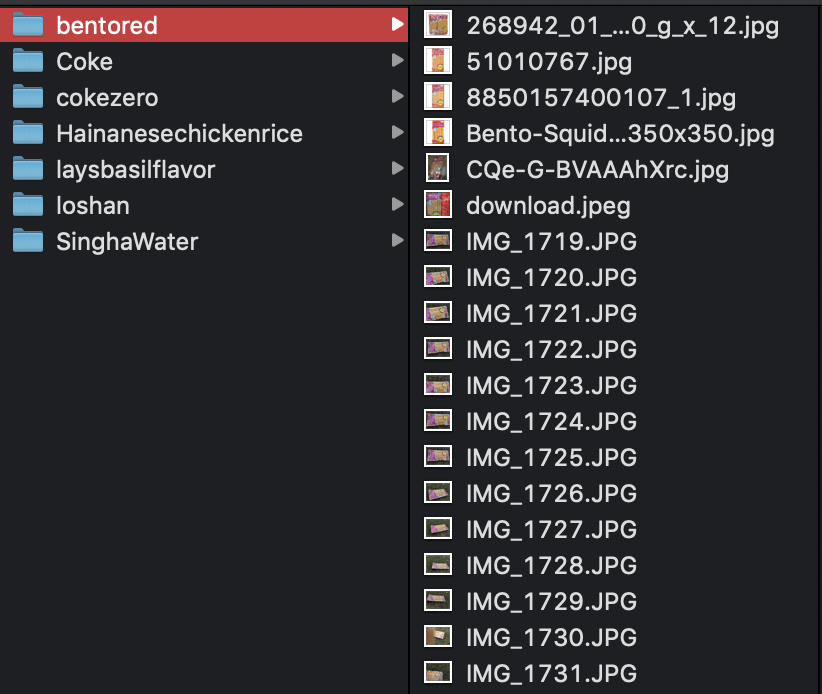
\includegraphics[width=0.8\textwidth]{Figures/3/ten/prepic.png}
								\caption{การเก็บข้อมูลภาพอาหาร}
								\label{Fig:picfood}
							\end{figure}
							จากภาพที่ \ref{Fig:picfood} สามารถอธิบายได้ดังนี้ินค้าแต่ละชนิดจะใช้ภาพจำนวน 100 ภาพในการฝึกฝน 
	

		\subsection{การตั้งค่าขนาดภาพและการใช้รูปแบบการจำแนก}
							ในขั้นตอนนี้จะทำการตั้งค่าขนาดภาพและเลือกใช้รูปแบบการจำแนก Mobilenet\_v1 โดยใช้คำสั่งเพื่อรันดังภาพที่ \ref{Fig:mobile}
			

\begin{figure}[H]
{\setstretch{1.0}\begin{lstlisting}
IMAGE_SIZE=224                  
ARCHITECTURE="mobilenet_v1_1.0_${IMAGE_SIZE}"
\end{lstlisting}}
\caption{คำสั่งการตั้งค่าขนาดภาพและการใช้รูปแบบการจำแนก}
\label{Fig:mobile}
\end{figure}
จากภาพที่ \ref{Fig:mobile} คำสั่งการตั้งค่าขนาดภาพและการใช้รูปแบบการจำแนก สามารถอธิบายการทำงานได้ดังนี้
\begin{itemize}[label={--}]
	\item บรรทัดที่  1	     เป็นการตั้งค่าขนาดของภาพเพื่ิอให้ภาพมีขนาดเท่ากัน
	\item บรรทัดที่  2 	     เป็นการเลือกใช้รูปแบบการจำแนกเพื่อทำการฝึกฝน  
\end{itemize}


	\subsection{การสร้างโมเดลด้วย Tensorflow Lite}
							ในขั้นตอนนี้จะทำการตั้งค่าขนาดภาพและเลือกใช้รูปแบบการจำแนก Mobilenet\_v1 โดยใช้คำสั่งเพื่อรันดังภาพที่ \ref{Fig:model}

\begin{figure}[H]
{\setstretch{1.0}\begin{lstlisting}
sudo python -m scripts.retrain \
--bottleneck_dir=tf_files/bottlenecks \
--how_many_training_steps=40000 \
--model_dir=tf_files/models/ \
--summaries_dir=tf_files/training_summaries/"${ARCHITECTURE}" \
--output_graph=tf_files/retrained_graph.pb \
--output_labels=tf_files/retrained_labels.txt \
--architecture="${ARCHITECTURE}" \
--image_dir=tf_files/test

\end{lstlisting}}
\caption{คำสั่งการตั้งค่าขนาดภาพและการใช้รูปแบบการจำแนก}
\label{Fig:model}
\end{figure}
\newpage




จากภาพที่ \ref{Fig:model} โครงสร้างขคำสั่งการตั้งค่าขนาดภาพและการใช้รูปแบบการจำแนกสามารถอธิบายการทำงานได้ดังนี้
\begin{itemize}[label={--}]
\item บรรทัดที่  1	     เป็นคำสั่งรันสคริปที่ทาง Google ได้ทำไว้
\item บรรทัดที่  2 	     เป็นคำสั่งสำหรับการเข้ารหัสรูปภาพ
\item บรรทัดที่  3       เป็นคำสั่งที่ระบุจำนวนของการฝึกฝน 
\item บรรทัดที่  4       เป็นคำสั่งระบุที่อยู่ของโมเดล 
\item บรรทัดที่  5       เป็นคำสั่งระบุที่อยู่ในการจัดเก็บผลลัพธ์จากการฝึกฝน
\item บรรทัดที่  6       เป็นคำสั่งระบุที่อยู่ในการ Export ไฟล์ retrained\_graph.PB 
\item บรรทัดที่  7       เป็นคำสั่งระบุที่อยู่ในการ Export ไฟล์ retrained\_labels.text 
\item บรรทัดที่  8       เป็นคำสั่งใช้งานรูปแบบการจำแนก
\item บรรทัดที่  9       เป็นคำสั่งระบุที่อยู่ของรูปภาพ
\end{itemize}
\subsection{การแปลไฟล์ PB ไปเป็น lite}
ในขั้นตอนนี้จะแปลงไฟล์ PB ไปเป็น lite เพื่อนำไปใช้กับแอนดรอย์แอปพลิเคชัน โดยใช้คำสั่งเพื่อรันดังภาพที่ \ref{Fig:convert}

\begin{figure}[H]
{\setstretch{1.0}\begin{lstlisting}
IMAGE_SIZE=224
tflite_convert \
--graph_def_file=tf_files/retrained_graph.pb \
--output_file=tf_files/optimized_graph.lite \
\end{lstlisting}}
\caption{คำสั่งในการแปลงไฟล์ PB ไปเป็น lite }
\label{Fig:convert}
\end{figure}
จากภาพที่ \ref{Fig:convert} คำสั่งการแปลงไฟล์ PB ไปเป็น lite สามารถอธิบายการทำงานได้ดังนี้
\begin{itemize}[label={--}]
\item บรรทัดที่  1	     เป็นการเรียกใช้สคริปสำหรับการแปลงไฟล์
\item บรรทัดที่  2 	     เป็นคำสั่งระบุที่อยู่ของไฟล์ PB 
\item บรรทัดที่  3       เป็นคำสั่งระบุที่จัดเก็บไฟล์ lite  
\end{itemize}



								
			